\section{Modellierung der Funktion}
\label{mdf}
In diesem Kapitel wird das eigentliche Data Mining in Form der Regressionsanalyse (vgl. \vref{fm}) angewendet, indem die zuvor selektierten, vorverarbeiteten und transformierten Daten mit Hilfe des MATLAB-Tools (vgl. \vref{matlab}) zu einer Funktion modelliert werden. Unter der Betrachtung des Winkels- und der Distanz des Schusses zum Tor (siehe \vref{bwd}) sowie unter der Betrachtung der Koordinaten des Schusses (siehe \vref{bk}) werden im Folgenden das \textit{multiple} und das \textit{nichtparametrische} Regressionsmodell (vgl. \vref{rm}) gegenübergestellt, um eine fundierte Grundlage für die Interpretation der Ergebnisse zu gewinnen.


\subsection{Betrachtung des Winkels- und der Distanz}
\label{bwd}
Die Daten wurden für die Betrachtung des Winkels- und der Distanz des Schussversuchs zuvor in \vref{wdt} in ein adaptiertes Format transformiert, sowie zu einer verwendbaren Datenmenge aggregiert. Diese Datenmenge wird zunächst in MATLAB importiert, sodass die einzelnen Variablen anschließend mit Hilfe des \gls{cft} (vgl. \vref{matra}) ausgewählt werden können, wie in \vref{auswahlWD} abgebildet.

\begin{figure}[H]
\centering
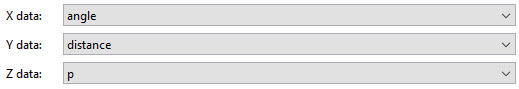
\includegraphics[scale=0.8]{se-wa-jpg/auswahlWD}
\caption{Auswahl der Daten für die Winkel- und Distanzbetrachtung im CFT}
\label{auswahlWD}
\end{figure}

Dabei gilt folgende Zuordnung, wobei Winkel und Distanz die unabhängigen und die Wahrscheinlichkeit die abhängige Variable bildet:

\begin{itemize}
\item Winkel $\rightarrow$  X-Achse
\item Distanz $\rightarrow$ Y-Achse
\item Wahrscheinlichkeit ($p$) $\rightarrow$ Z-Achse
\end{itemize}

Die Wertebereiche der Variablen (gleiches gilt für die Achsen) sind aus der Transformation in \vref{wdt} zu übernehmen und entsprechend über den Tab \textit{Tools}$\rightarrow$\textit{Axis Limits} einzutragen.

\begin{itemize}
\item $ 0 \le$ Winkel $\le 90$
\item $ 1 \le$ Distanz $\le 100$
\item $ 0 \le$ Wahrscheinlichkeit $\le 1$
\end{itemize}

Stellt man die aggregierten Daten ohne eine angepasste Funktion dar, ergibt sich \vref{rowWD}, wobei die vorherige Einteilung der Daten in Raster deutlich wird. Jeder orangefarbene Punkt repräsentiert dabei in der Höhe die Wahrscheinlichkeit in Form der relativen Häufigkeit. Bereits in dieser vereinfachten Abbildung wird deutlich, dass ab einer bestimmten Distanz (ca. \textsf{40}) der Winkel keinen Einfluss mehr auf die Wahrscheinlichkeit eines Torerfolges hat. Mit Hilfe des \textit{multiplen} und des \textit{nichtparametrischen} Regressionsmodelles soll nachfolgend eine Funktion modelliert werden, die diese Punktewolke bestmöglich beschreibt, wobei das Bestimmtsheitsmaß (vgl. \vref{bhm}) eine objektive Aussage über die Anpassung des Modells an die Daten bietet.

\begin{figure}[H]
\centering
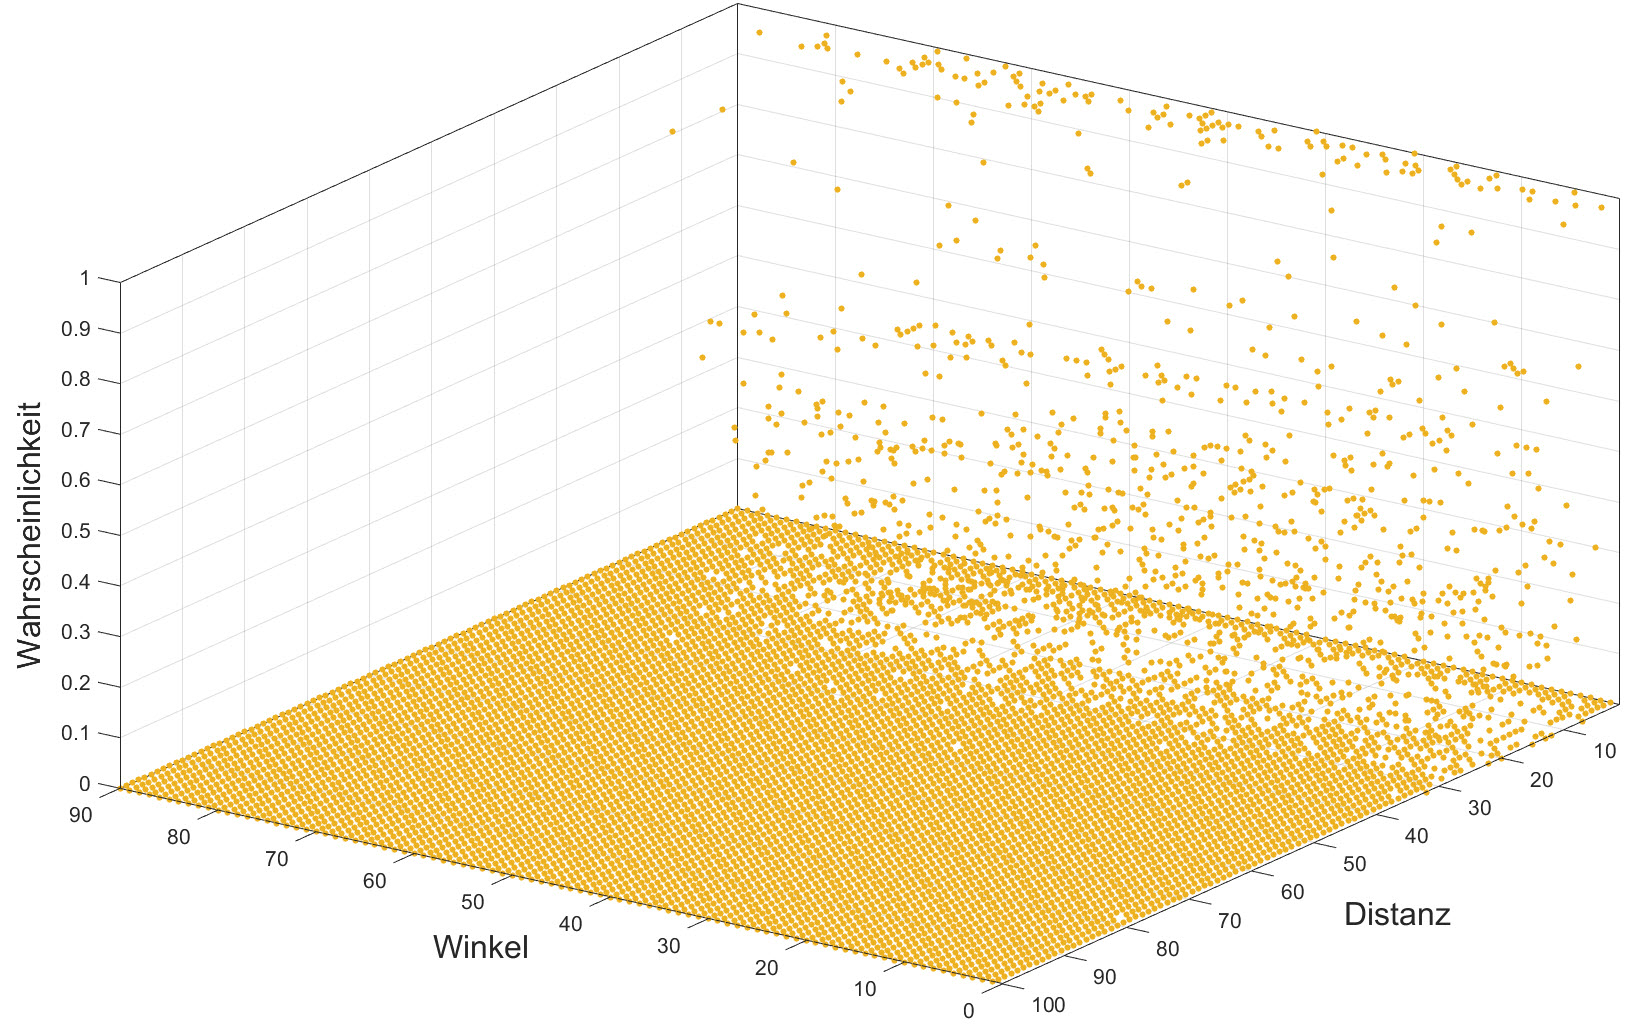
\includegraphics[scale=0.345]{se-wa-jpg/rowWD}
\caption{Darstellung der transformierten Daten der Winkel- und Distanzbetrachtung}
\label{rowWD}
\end{figure}

Betrachtet man die Wahrscheinlichkeit eines Torerfolges in Abhängigkeit von der Distanz, wie in \vref{outlierWD} dargestellt, so lassen sich Ausreißer -- wie der Rekordschuss von Moritz Stoppelkamp (vgl. \vref{datac}) -- schnell erkennen und über das CFT von der Berechnung ausschließen. Dieser Schritt ist essenziell für die Modellierung, da die stark von der Grundmenge abweichenden Daten die Funktion deutlich beeinflussen und damit die Realität verzerren.

\begin{figure}[H]
\centering
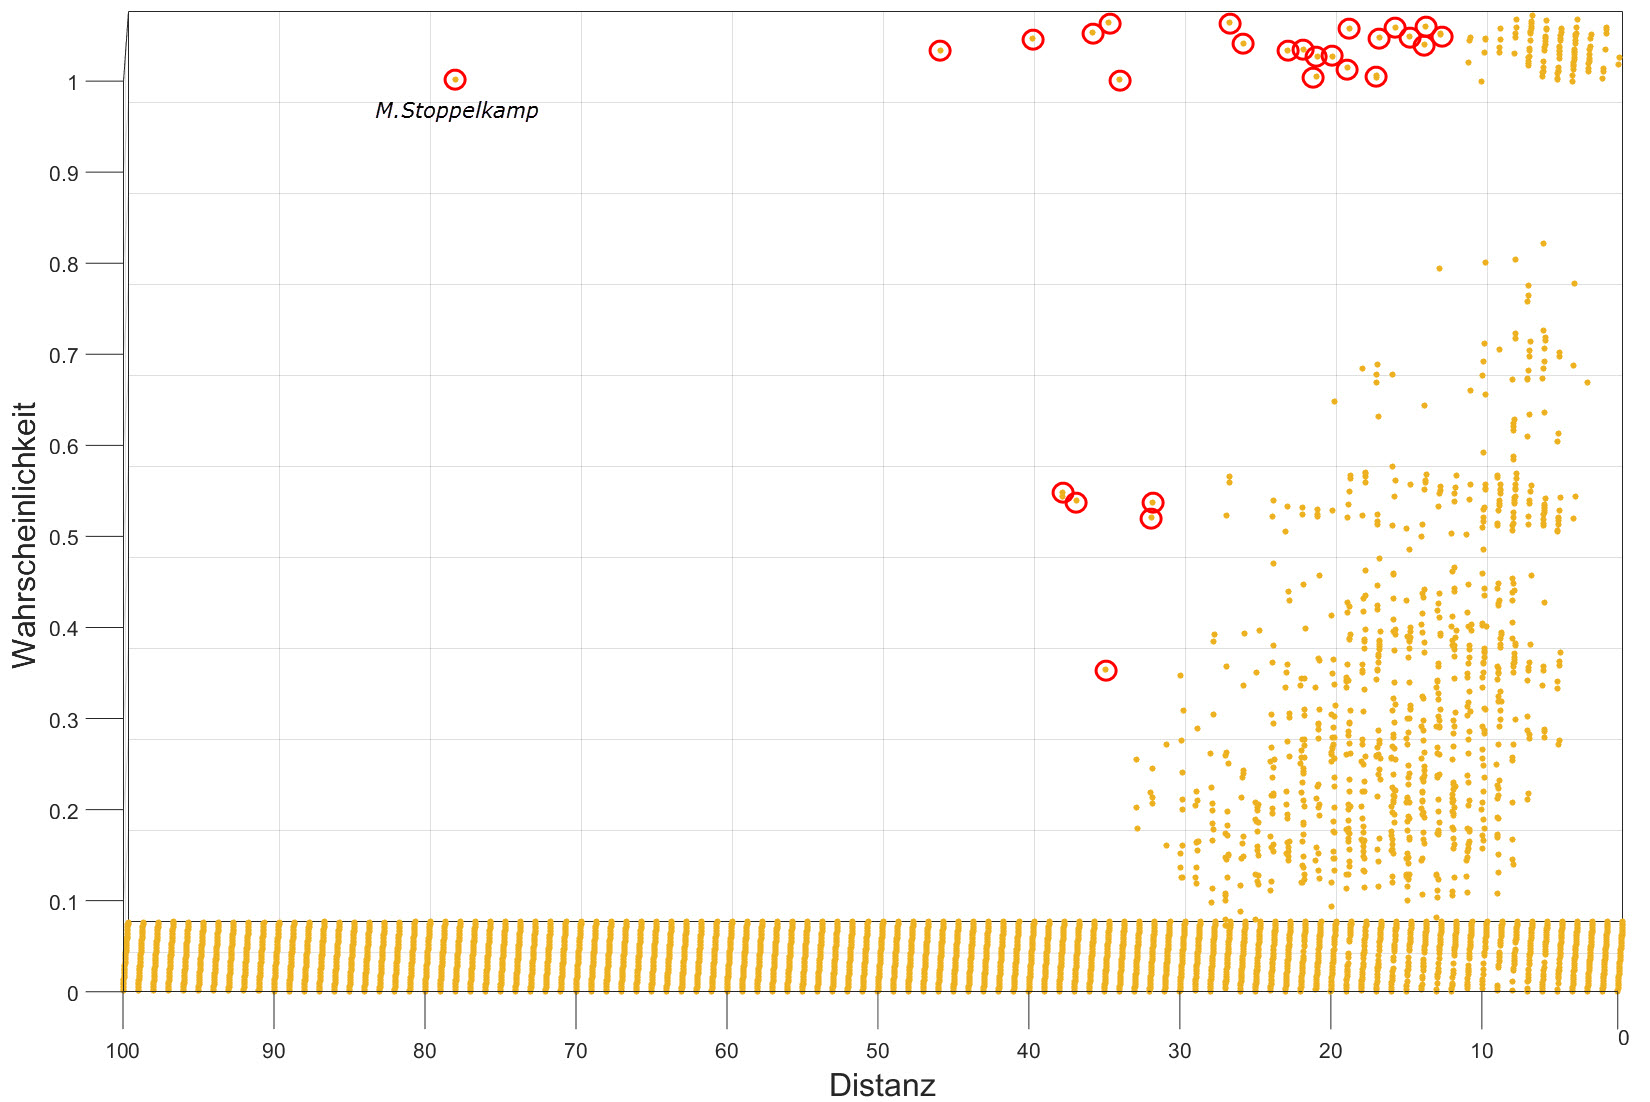
\includegraphics[scale=0.33]{se-wa-jpg/outlierWD}
\caption{Ausreißererkennung der Winkel- und Distanzbetrachtung}
\label{outlierWD}
\end{figure}

\subsubsection{Multiple Regression}
Wie in \vref{rm} beschrieben, wird die \textit{multiple} Regression für Anwendungsfälle genutzt, bei denen die Zielvariable von mehreren unabhängigen Variablen abhängig ist, wie in diesem Fall von dem Winkel und der Distanz des Schusses zum Tor. Da es sich um ein parametrisches Regressionsmodell handelt, muss zwingend eine Funktion vorgegeben werden. Innerhalb der Regressionsanalyse werden dann die Parameter so justiert, dass die Funktion möglichst genau an die Daten angepasst werden kann. Im CFT wird dazu, wie in \vref{polyWD} abgebildet, der Funktionstyp \textit{Polynomial} mit den Polynomgraden \textsf{5} für die unabhängigen Variablen ausgewählt. Der Funktionstyp \textit{Lowess} modelliert die Funktion mit \textit{Splines} (vgl. \vref{rm}) und wird innerhalb der \textit{nichtparametrischen} Regression verwendet (siehe \vref{wdnr}). Das Verfahren der Interpolation beschreibt jeden Punkt als eine eigene stetige Funktion und bildet damit sogenannte \textit{Peaks}, welche im Anhang in \vref{inter} betrachtet werden können.\enlargethispage{\baselineskip} Eine benutzerdefinierte Gleichung kann ebenfalls ausgeschlossen werden, da in diesem Prozess viele mathematische Annahmen und Vermutungen getroffen werden müssen, sodass diese Möglichkeit aufgrund der zeitlichen Ressourcen nicht zu realisieren ist.

\begin{figure}[H]
\centering
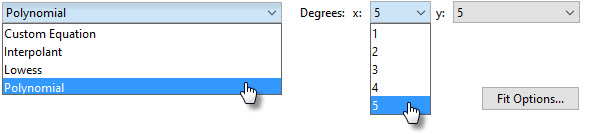
\includegraphics[scale=0.8]{se-wa-jpg/polyWD}
\caption{Auswahl der multiplen Regressionsfunktion}
\label{polyWD}
\end{figure}

Wie zu erkennen ist, unterstützt MATLAB die Polynomfunktionen bis zum fünften Grad, welcher für die \textit{multiple} Regression ausgewählt wird, da ein höherer Grad eine bessere Anpassung an die Daten verspricht. Das Ergebnis dazu lässt sich in \vref{plotWD} betrachten.

\begin{figure}[H]
\centering
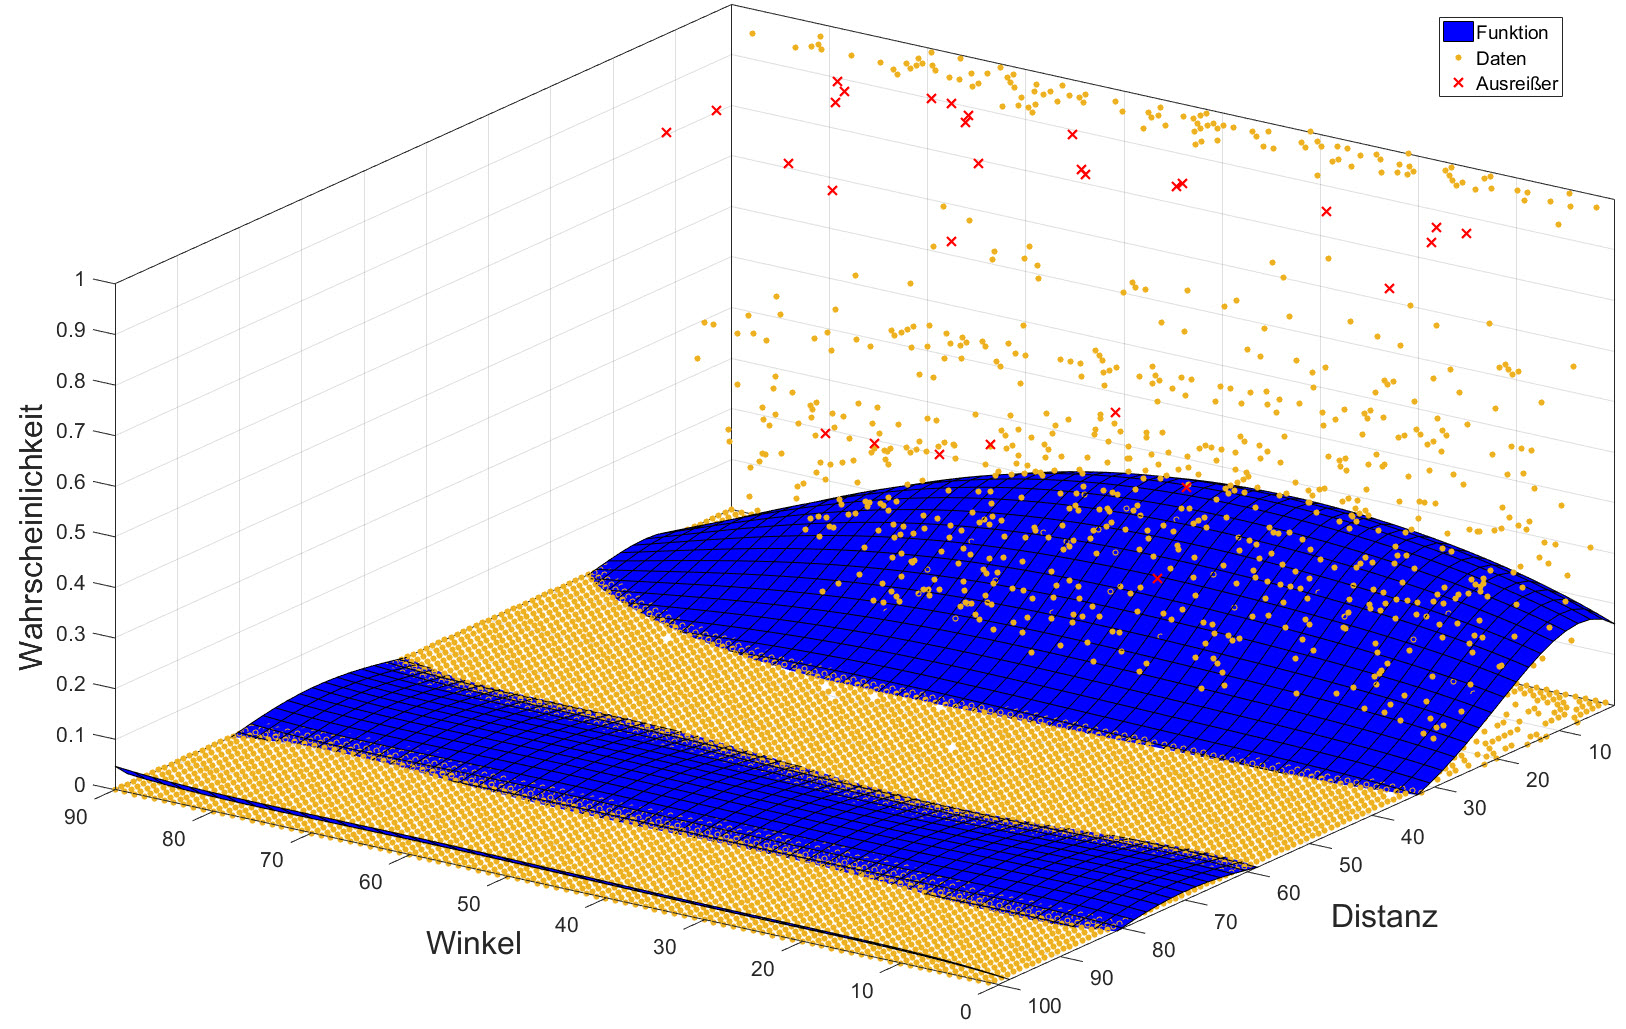
\includegraphics[scale=0.34]{se-wa-jpg/plotWD}
\caption{Multiple Regressionsfunktion der Winkel- und Distanzbetrachtung}
\label{plotWD}
\end{figure}

Die Polynomfunktion ist sehr glatt modelliert und geht teilweise sogar in den negativen Wertebereich der Wahrscheinlichkeit, wie beispielsweise zwischen den Distanzen \textsf{40} und \textsf{60}. Diese Tatsache ist aus Sicht des Sinnes der Daten nicht tragbar, da große Flächen der Funktion eine negative Wahrscheinlichkeit repräsentieren, welche in der Realität nicht existieren können und folglich auch nicht im Modell. Die Bestimmtheitsmaße aus \vref{tab:gofmrwd} bestätigen diesen Eindruck mit relativ schlechten Werten für die Anpassung des Modelles an die Daten.

%%%%%%%%%%%%%%%%%% Tabelle GOFMRWD %%%%%%%%%%%%%%%%%%
\tablefirsthead{\hline\multicolumn{2}{|c|}{\textbf{Goodness of Fit}}\\\hline}
\tablehead{}
\tabletail{}
\tablelasttail{}
\bottomcaption{Goodness of Fit der multiplen Regression der Winkel- und Distanzbetrachtung\label{tab:gofmrwd}}
\begin{center}%
\begin{supertabular}{ | P{6cm} | P{3cm}  |}
\textsf{R-Qudrat} 	& 0.3061	\\
\hline
\textsf{korrigiertes R-Qudrat} 	&  0.3045	\\
\hline
\end{supertabular}
\end{center}

\subsubsection{Nichtparametrische Regression}
\label{wdnr}
Da sich von vornherein nur schwer eine Regressionsfunktion mit bestimmter Spezifizierung der Parameter vorhersagen lässt, wird auf die \textit{nichtparametrische} Regression in Form der von MATLAB bereitgestellten \gls{lowess}- Methode zurückgegriffen. Die x-(\textit{Winkel}) und y-(\textit{Distanz})-Werte werden dabei in eine feines Gitter -- ähnlich der Rastereinteilung innerhalb der Transformation -- eingeteilt und diese Bereiche einzeln durch Polynome niedrigen Grades beschrieben. Durch die Aneinanderreihung der Gitter an den \glqq Knotenpunkten\grqq~lässt sich die gesuchte Funktion schätzen. Bei der Auswahl der \gls{lowess}-Methodik (siehe \vref{span}) kann dabei mit Hilfe des \textit{Span}-Parameters die Glättung der Funktion bestimmt werden. Dieser gibt prozentual (zwischen 1 bis 100\%) an, wie viele Datenpunkte zur lokalen Regression herangezogen werden. Das bedeutet wie groß das Gitter im Verhältnis zur gesamten Datenmenge gestrickt werden soll. Wird der Span-Wert reduziert, passt sich die Funktion sehr nah an die Daten an, wobei eine Erhöhung des Span-Wertes im Gegensatz dazu zu einer starken Glättung der Funktion führt.\seFootcite{Vgl.}{}{matlab.2017}

\begin{figure}[H]
\centering
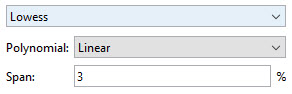
\includegraphics[scale=0.9]{se-wa-jpg/span}
\caption{Auswahl der Lowess Methode und Bestimmung des Span-Wertes}
\label{span}
\end{figure}

In \vref{splinewd} ist die \textit{nichtparametrische} Regressionsfunktion mit einem Span-Wert von \textsf{3} dargestellt, wobei die Fläche der negativen Wahrscheinlichkeiten gegenüber der \textit{multiplen} Regression hier sehr gering ist und die Fläche nicht zu stark geglättet, jedoch auch nicht zu rau ist. Der Span-Wert muss dabei so gewählt werden, dass eine Balance zwischen \textbf{Underfitting} und \textbf{Overfitting} \vref{bhm}) gefunden wird und der Sinn der Daten dabei nicht verloren geht. Im Anhang befindet sich dazu jeweils ein Beispiel bei einer zu kleinen (vgl. \vref{splinewdTM}) bzw. zu großen Verwendung (vgl. \vref{splinewdTL}) des Span-Wertes.

\begin{figure}[H]
\centering
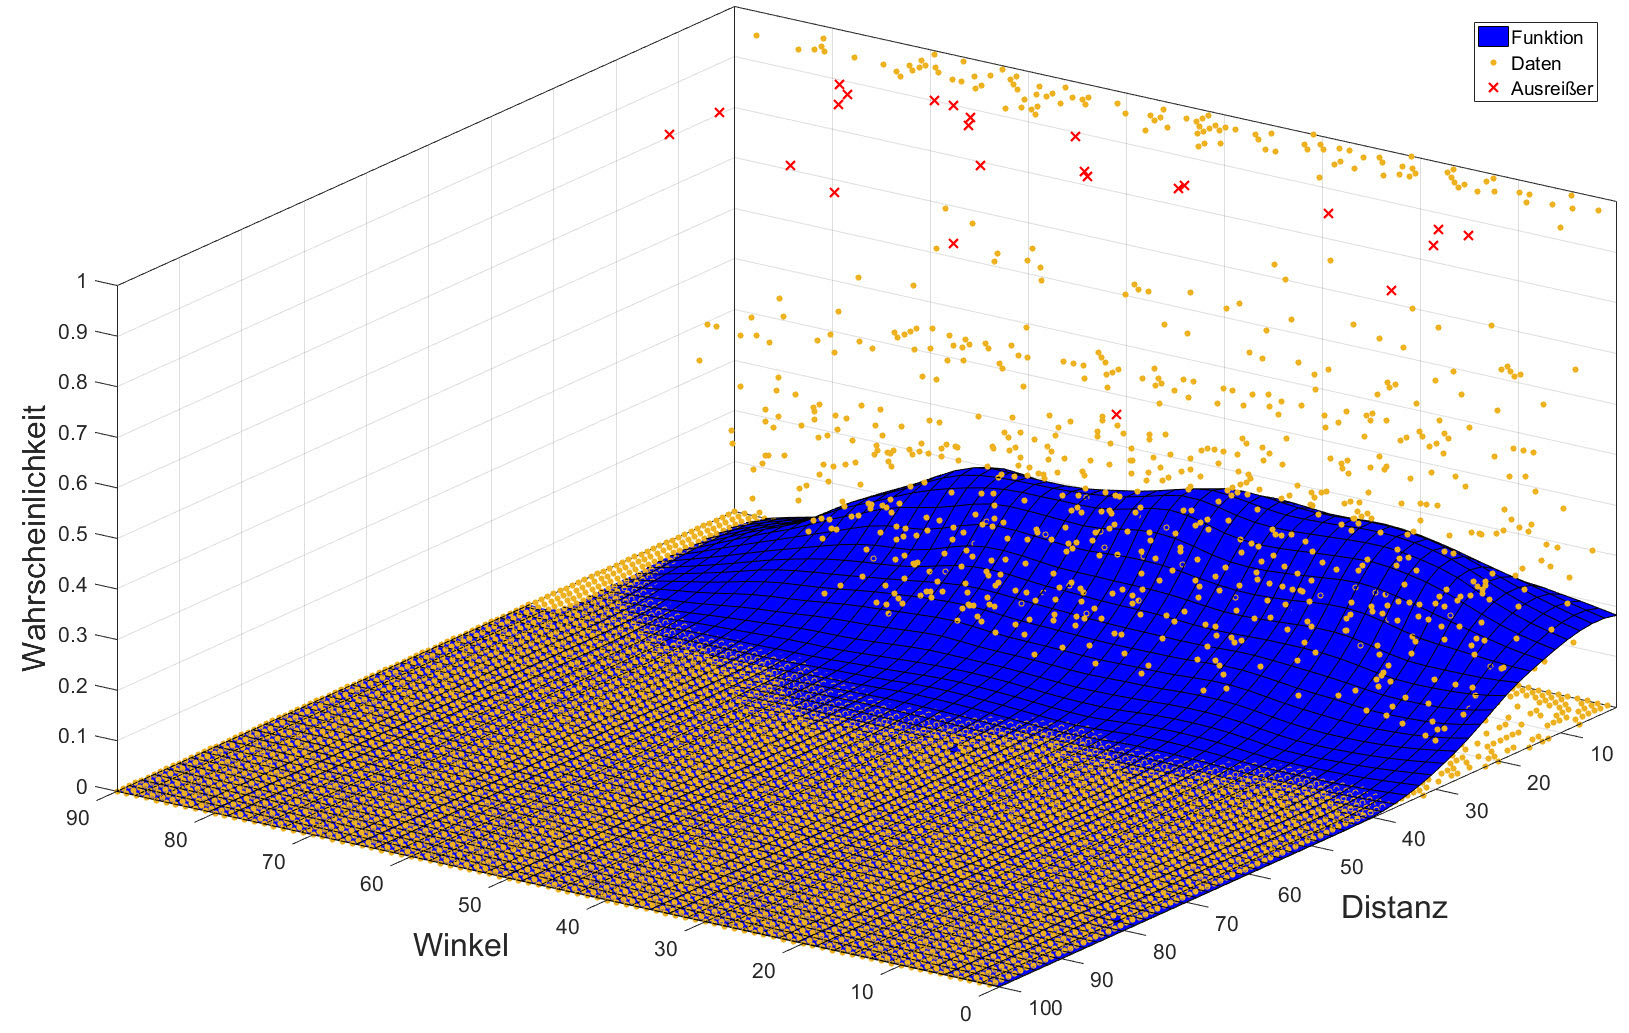
\includegraphics[scale=0.34]{se-wa-jpg/splinewd}
\caption{Lowess-Funktion der Winkel- und Distanzbetrachtung}
\label{splinewd}
\end{figure}

\enlargethispage{2\baselineskip} Die Bestimmtheitsmaße der \textit{nichtparametrische} Regressionsfunktion aus \vref{tab:gofnrwd} sind gegenüber der \textit{multiplen} Regression im Schnitt um circa \textsf{0.1} gestiegen, jedoch befindet sich der Grad der Anpassung der Funktion an die Daten nach wie vor in einem inakzeptablen Bereich. Eine Erhöhung des Span-Wertes würde zu einem besseren Bestimmtheitsmaß führen, allerdings würde demzufolge auch ein Overfitting entstehen, da jeder Datenpunkt wiederum einzeln betrachtet wird und kein allgemeingültiges Modell resultieren würde.

%%%%%%%%%%%%%%%%%% Tabelle GOFNRWD %%%%%%%%%%%%%%%%%%
\tablefirsthead{\hline\multicolumn{2}{|c|}{\textbf{Goodness of Fit}}\\\hline}
\tablehead{}
\tabletail{}
\tablelasttail{}
\bottomcaption{Goodness of Fit der nichtparametrischen Regression der Winkel- und Distanzbetrachtung\label{tab:gofnrwd}}
\begin{center}%
\begin{supertabular}{ | P{6cm} | P{3cm}  |}
\textsf{R-Qudrat} 	& 0.4317	\\
\hline
\textsf{korrigiertes R-Qudrat} 	&  0.4187	\\
\hline
\end{supertabular}
\end{center}

%%%%%%%%%%%%%%%%%%%%%%%%%%%%%%%%%%%%%%%%%%%%%%%%%%%%%%%%%%%%%%%%%%%%%%%%%%%%%%%%%%%%%%
%%%%%%%%%%%%%%%%%%%%%%%%%%%%%%%%%%%%%%%%%%%%%%%%%%%%%%%%%%%%%%%%%%%%%%%%%%%%%%%%%%%%%%
%%%%%%%%%%%%%%%%%%%%%%%%%%%%%%%%%%%%%%%%%%%%%%%%%%%%%%%%%%%%%%%%%%%%%%%%%%%%%%%%%%%%%%

\subsection{Betrachtung der Koordinaten}
\label{bk}


In \vref{kt} wurden die Daten in ein adaptiertes Format für die Koordinatenbetrachtung transformiert, sowie zu einer verwendbaren Datenmenge, in Form von Rastern (vgl. \vref{raster}), aggregiert. Nach dem Import dieser spezifischen Datenmenge in MATLAB, können die einzelnen Variablen anschließend mit Hilfe des \gls{cft} (vgl. \vref{matra}) ausgewählt werden, wie in \vref{auswahlK} dargestellt.

\begin{figure}[H]
\centering
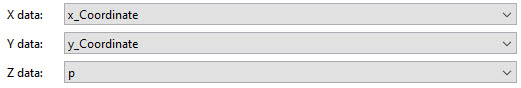
\includegraphics[scale=0.8]{se-wa-jpg/auswahlK}
\caption{Auswahl der Daten für die Koordinatenbetrachtung im CFT}
\label{auswahlK}
\end{figure}

Dabei gilt folgende Zuordnung, wobei die x- und y-Koordinate die unabhängigen und die Wahrscheinlichkeit die abhängige Variable bildet:

\begin{itemize}
\item x-Koordinate $\rightarrow$  X-Achse
\item y-Koordinate $\rightarrow$ Y-Achse
\item Wahrscheinlichkeit ($p$) $\rightarrow$ Z-Achse
\end{itemize}

Die Wertebereiche der Variablen und der Achsen wird aus der Transformation in \vref{kt} übernommen und analog in MATLAB eingetragen.

\begin{itemize}
\item $ -50 \le$ x-Koordinate $\le 50$
\item $ 1 \le$ y-Koordinate $\le 100$
\item $ 0 \le$ Wahrscheinlichkeit $\le 1$
\end{itemize}

\enlargethispage{2\baselineskip} Parallel zur Winkel- und Distanzbetrachtung werden die aggregierten Daten ohne eine angepasste Funktion zunächst in \vref{rowK} dargestellt, wobei hier ebenfalls die vorherige Einteilung der Daten in Raster deutlich wird. Zur besseren Vorstellung wurden dazu die Linien des Spielfeldes eingezeichnet. Das eigene Tor ist dabei bei $P_{ET}(0,100)$ und das gegnerische Tor bei $P_{GT}(0,0)$ platziert, woraus sich die Spielrichtung von $y=100 \rightarrow y=0$ ergibt. Die Wahrscheinlichkeit steigt dabei mit zunehmender Annäherung zum Tor und bildet im Strafraum des Gegners eine Art \glqq Gipfel\grqq.

\begin{figure}[H]
\centering
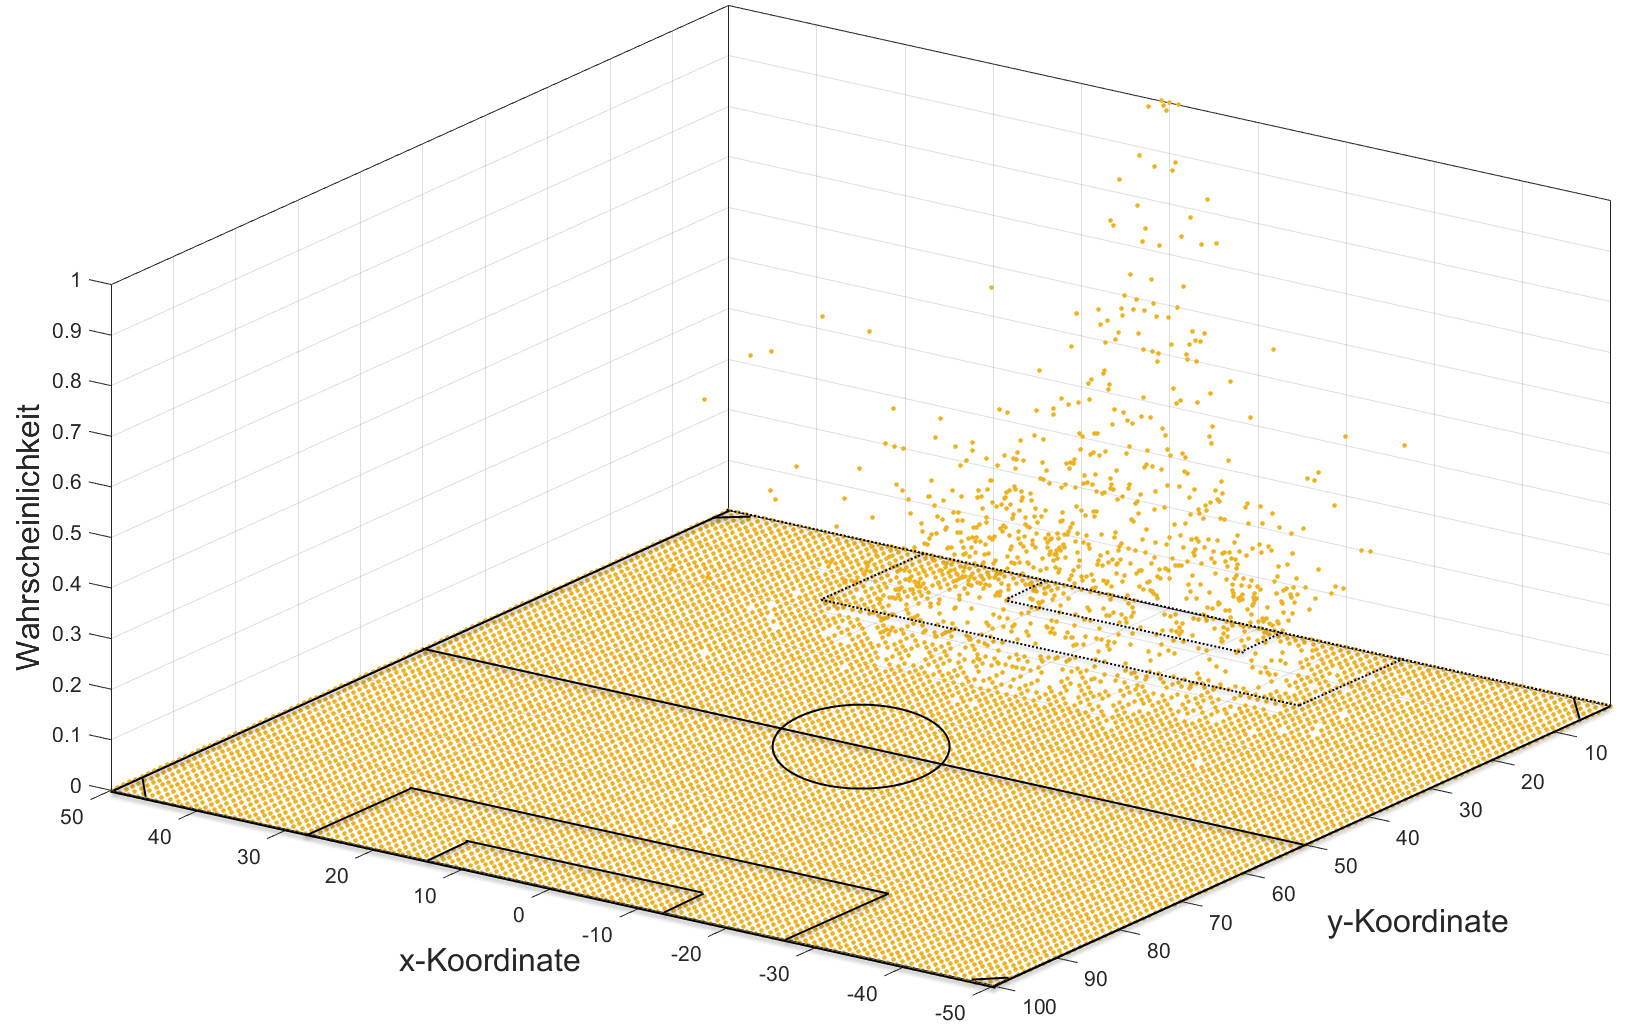
\includegraphics[scale=0.345]{se-wa-jpg/rowK}
\caption{Darstellung der transformierten Daten der Koordinatenbetrachtung}
\label{rowK}
\end{figure}

Bevor die Funktion mittels des \textit{multiplen} und des \textit{nichtparametrischen} Regressionsmodells modelliert werden kann, müssen zuvor die Ausreißer, wie beispielsweise der Rekordschuss von Moritz Stoppelkamp (vgl. \vref{datac}), von der Berechnung ausgeschlossen werden. Dazu werden sowohl in Bezug zu den Werten der x-Koordinate (siehe \vref{outlierKX}) als auch zu den Werten der y-Koordinate (siehe \vref{outlierKY}) die Ausreißer mit Hilfe der bereitgestellten Funktionalität in MATLAB markiert.

\begin{figure}[H]
\centering
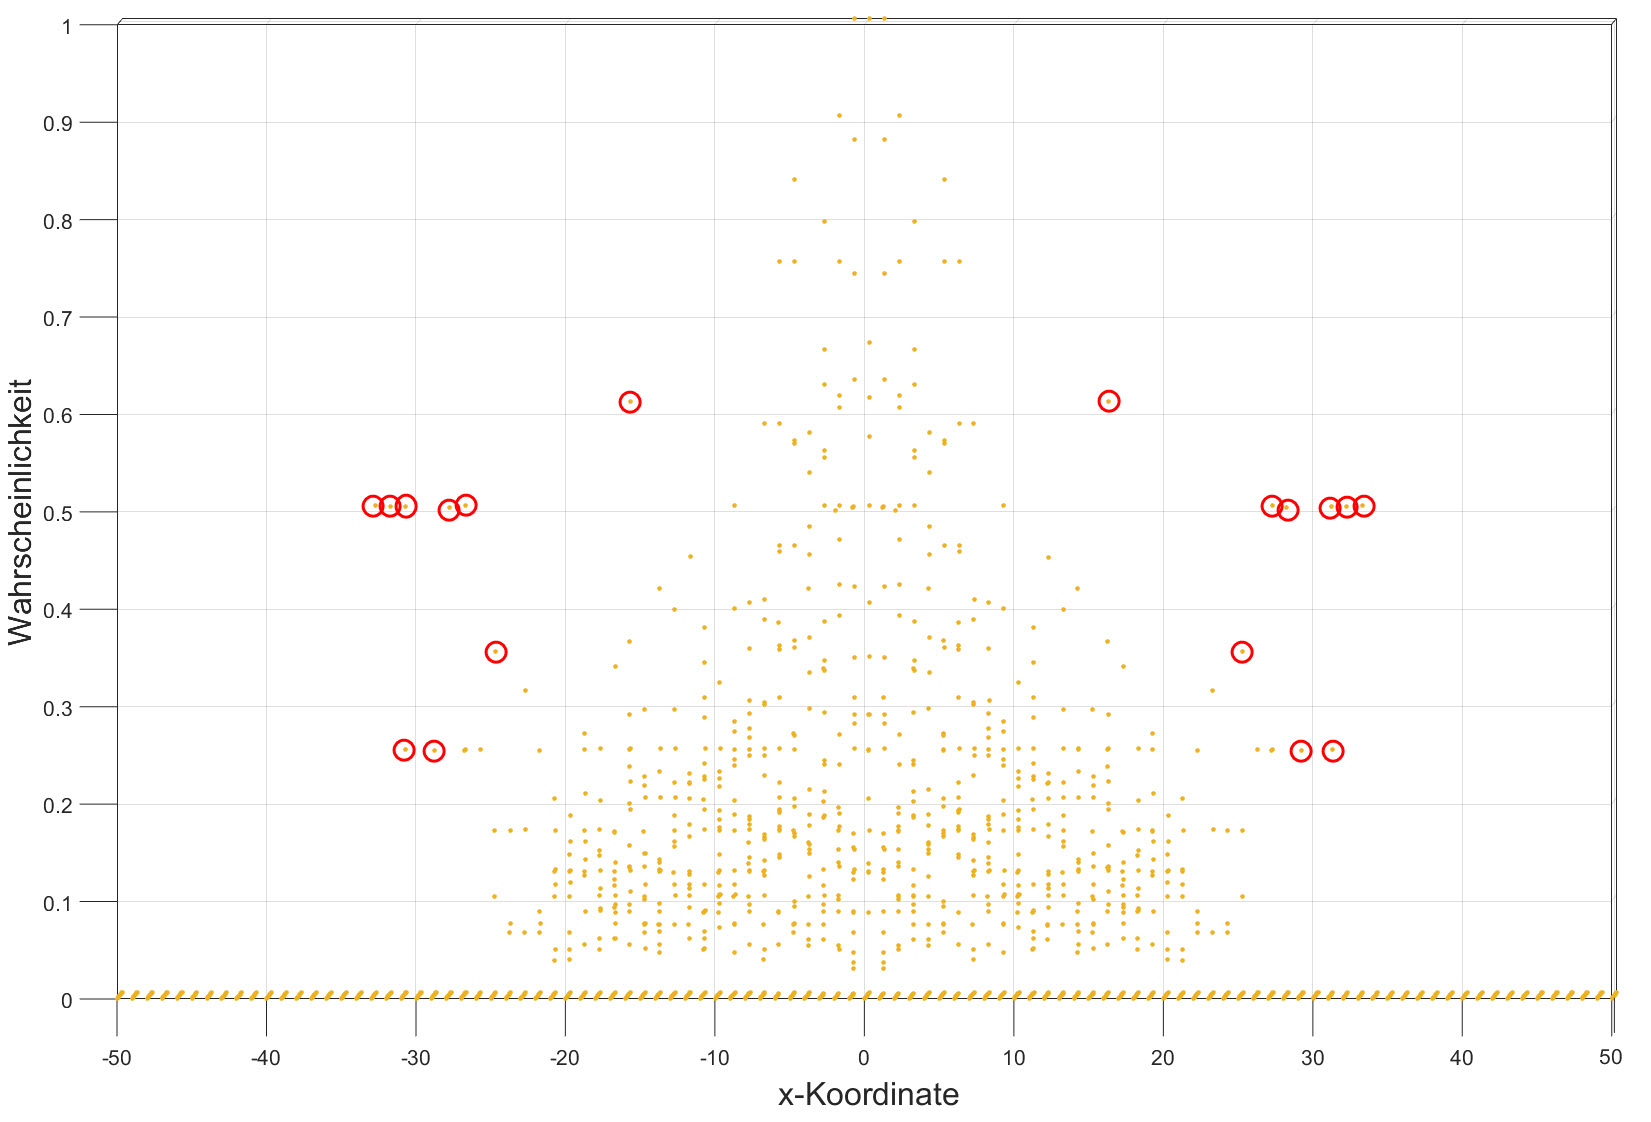
\includegraphics[scale=0.31]{se-wa-jpg/outlierKY}
\caption{Ausreißererkennung bei der Koordinatenbetrachtung (X-Koordinate)}
\label{outlierKX}
\end{figure}

\begin{figure}[H]
\centering
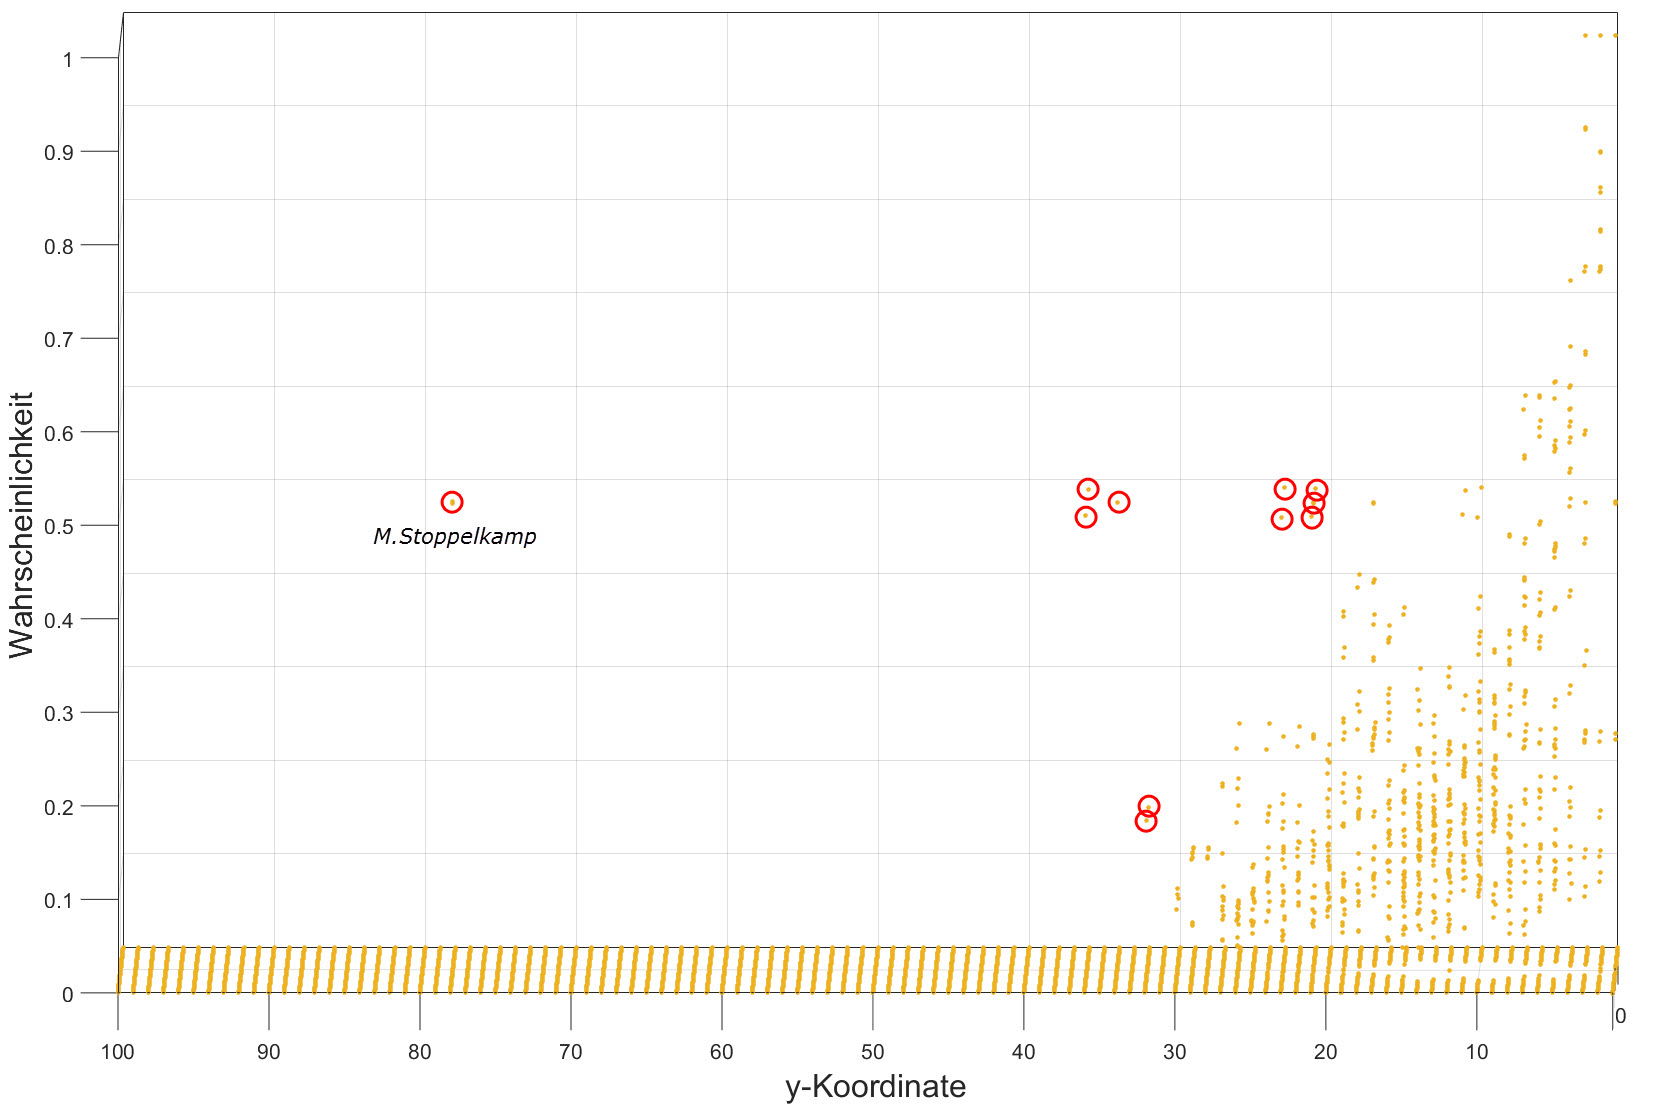
\includegraphics[scale=0.31]{se-wa-jpg/outlierKX}
\caption{Ausreißererkennung bei der Koordinatenbetrachtung (Y-Koordinate)}
\label{outlierKY}
\end{figure}

\subsubsection{Multiple Regression}

Wie bereits bei der Betrachtung des Winkels- und der Distanz des Schussversuches zum Tor (vgl. \vref{polyWD}), wird auch für die \textit{multiple} Regression in Bezug auf die Koordinaten des Schusses eine Polynomfunktion fünften Grades verwendet. Das daraus resultierende Ergebnis (siehe \vref{plotK}) ist dabei der zu Beginn vermuteten Funktion aus \vref{vermutung} sehr ähnlich, zumindest im Bereich des gegnerischen Strafraums. Jedoch liegen große Flächen der Funktion hierbei ebenfalls im negativen Bereich der Wahrscheinlichkeit, welche durch die orangefarbenen Bereiche erkannt werden können. Des Weiteren steigt die Wahrscheinlichkeit an den Seitenlinien des Spielfeldes ($x=50$ bzw. $x=-50$), sowie seitlich des eigenen Strafraums ($20 \le x \le 40$ und $-20 \le x \le 20)$, was wiederum nicht der Realität entspricht und der Form der Polynomfunktion geschuldet ist.

\begin{figure}[H]
\centering
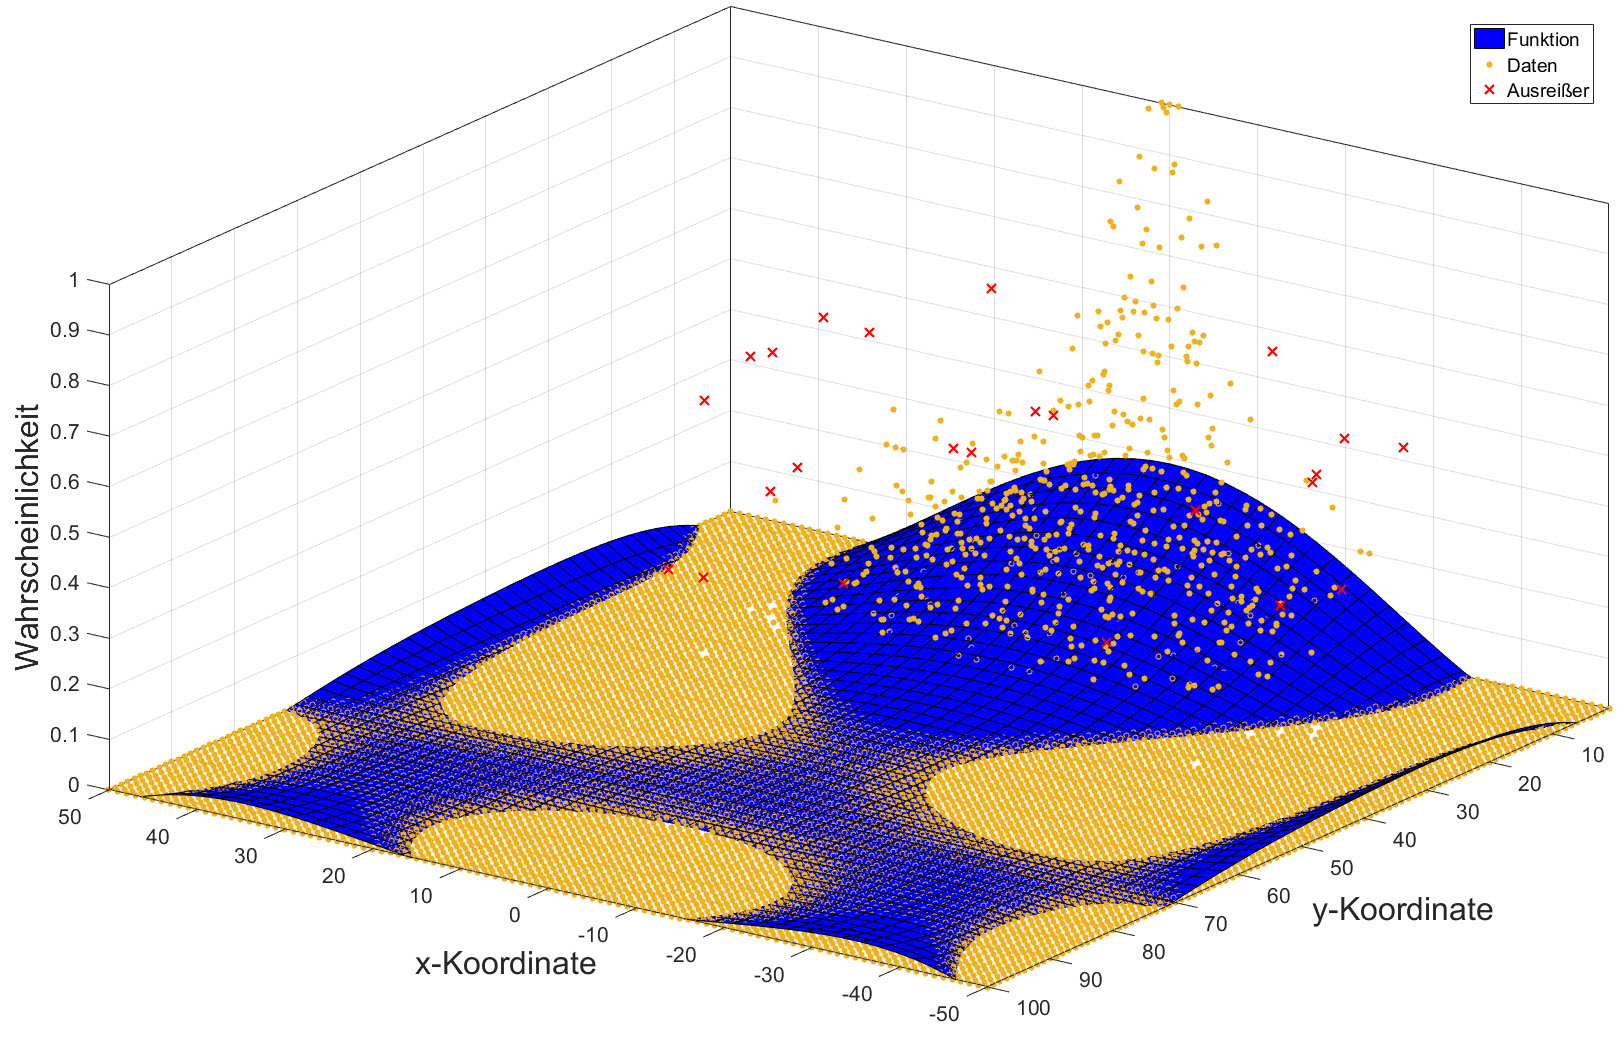
\includegraphics[scale=0.34]{se-wa-jpg/plotK}
\caption{Multiple Regressionsfunktion der Koordinatenbetrachtung}
\label{plotK}
\end{figure}

Die Bestimmtheitsmaße dieser Modellierung aus \vref{tab:gofmrk} bestärken in einer objektiven Größe diese Mängel der Funktion. Ein weiterer Kritikpunkt stellen Schussversuche aus spitzem Winkel dar, beispielsweise ein Schuss von der Position $x=20$ und $y=2$, die in diesem Modell aufgrund der starken Glättung eine zu hohe Wahrscheinlichkeit widerspiegeln. In \vref{heatmap} (a) wird diese Besonderheit durch die Visualisierung der Wahrscheinlichkeit anhand einer Heatmap deutlich. Um das gegnerische Tor bildet sich eine Art Halbkreis, sodass der genannte Schussversuch mit der gleichen Wahrscheinlichkeit eingestuft wird, wie ein Schussversuch von zentraler Position außerhalb des Strafraums, obwohl der Winkel ($84^\circ$ vgl. \vref{winkel_distanz}) zum Tor sehr spitz ist.

%%%%%%%%%%%%%%%%%% Tabelle GOFMRK %%%%%%%%%%%%%%%%%%
\tablefirsthead{\hline\multicolumn{2}{|c|}{\textbf{Goodness of Fit}}\\\hline}
\tablehead{}
\tabletail{}
\tablelasttail{}
\bottomcaption{Goodness of Fit der multiplen Regression der Koordinatenbetrachtung\label{tab:gofmrk}}
\begin{center}%
\begin{supertabular}{ | P{6cm} | P{3cm}  |}
\textsf{R-Qudrat} 	& 0.4981	\\
\hline
\textsf{korrigiertes R-Qudrat} 	&  0.4971	\\
\hline
\end{supertabular}
\end{center}

\subsubsection{Nichtparametrische Regression}

Zur Umsetzung der \textit{nichtparametrischen} Regression wird wie innerhalb der Winkel- und Distanzbetrachtung (vgl. \vref{span}) die \gls{lowess}-Methode mit einem Span-Wert von \textsf{3\%} verwendet. Mit diesem Wert konnte eine gute Balance zwischen einem Under- bzw. Overfitting des Modelles erreicht werden. Dieser wurde letztlich durch mehrere iterative Annäherungen als optimalen Wert ausgewählt, wozu\enlargethispage{2\baselineskip} das Ergebnis dieser Modellierung in \vref{splinek} abgebildet ist.

\begin{figure}[H]
\centering
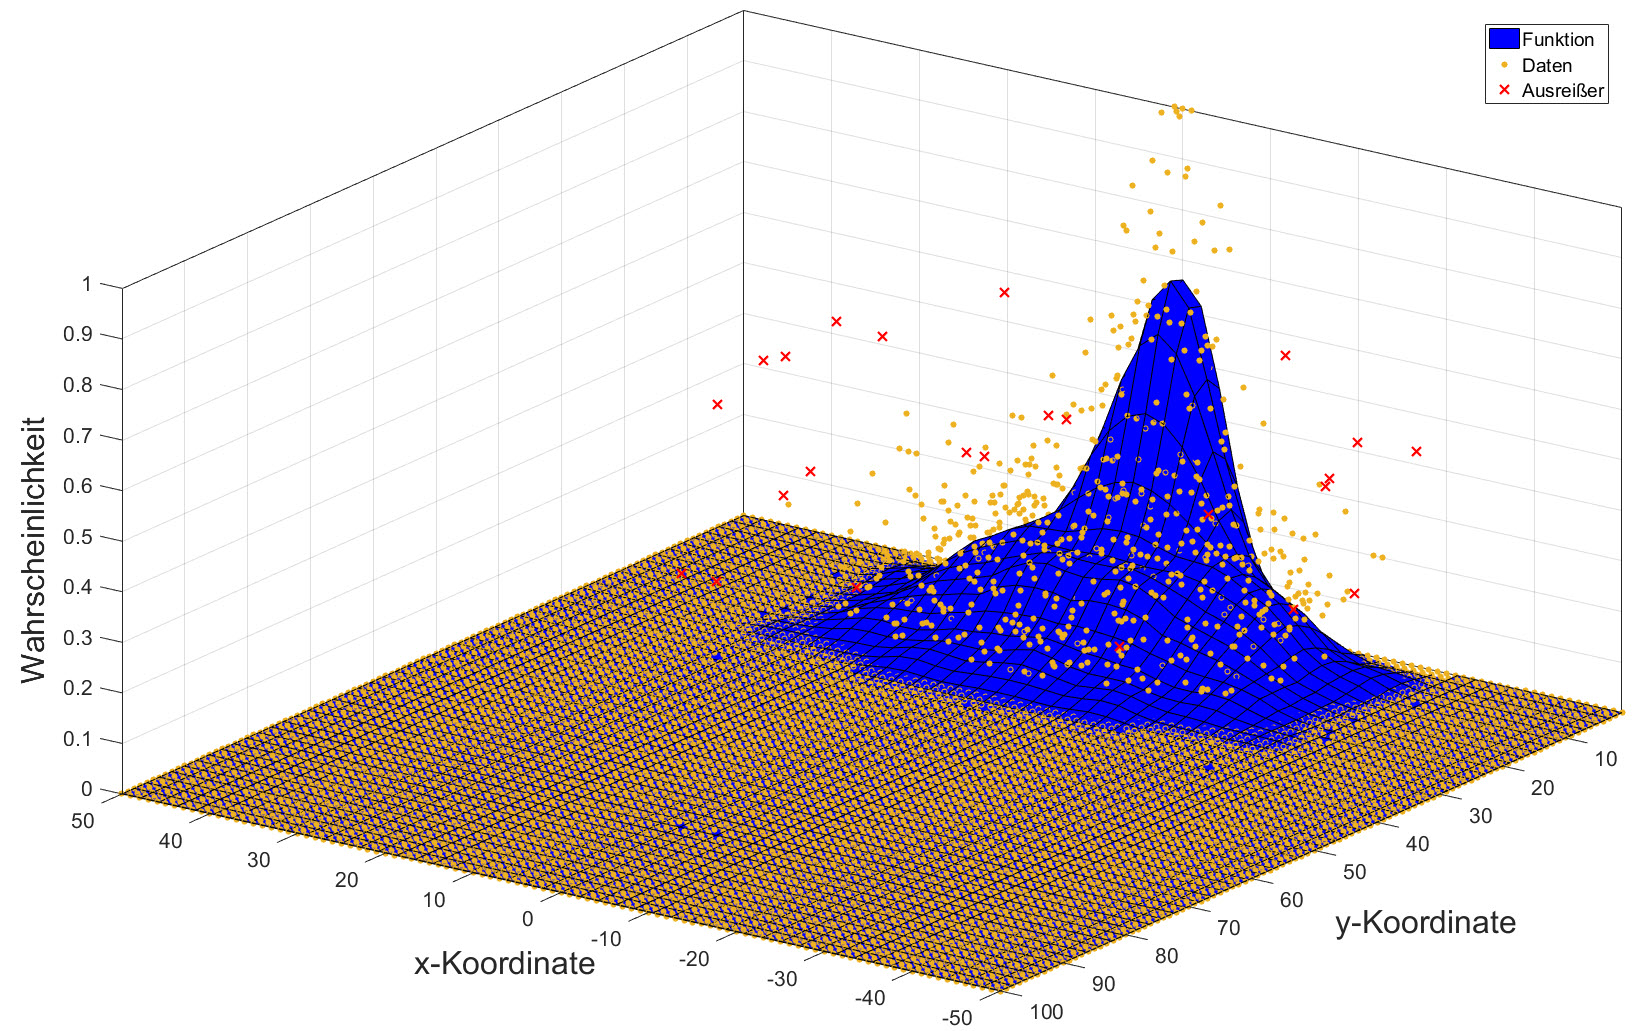
\includegraphics[scale=0.34]{se-wa-jpg/splinek}
\caption{Lowess-Funktion der Koordinatenbetrachtung}
\label{splinek}
\end{figure}

Aus der Abbildung lässt sich entnehmen, dass die Funktion innerhalb der angegebenen Wertebereiche keine negativen Wahrscheinlichkeiten annimmt, sowie den Bereich des gegnerischen Strafraums relativ exakt modelliert, wodurch der angesprochene \glqq Gipfel\grqq~ widergespiegelt wird. \vref{tab:gofnrk} bestätigt diese Annahmen mit sehr guten Werten der Bestimmtheitsmaße, die für eine genaue Anpassung des Modelles an die Daten sprechen.

%%%%%%%%%%%%%%%%%% Tabelle GOFNRK %%%%%%%%%%%%%%%%%%
\tablefirsthead{\hline\multicolumn{2}{|c|}{\textbf{Goodness of Fit}}\\\hline}
\tablehead{}
\tabletail{}
\tablelasttail{}
\bottomcaption{Goodness of Fit der nichparametrischen Regression der Koordinatenbetrachtung\label{tab:gofnrk}}
\begin{center}%
\begin{supertabular}{ | P{6cm} | P{3cm}  |}
\textsf{R-Qudrat} 	& 0.7761	\\
\hline
\textsf{korrigiertes R-Qudrat} 	&  0.7715	\\
\hline
\end{supertabular}
\end{center}

Das innerhalb der \textit{multiplen} Regression angesprochene Problem der verfälschten Wahrscheinlichkeit eines Schussversuches aus spitzem Winkel, tritt in der \textit{nichtparametrischen} Modellierung nicht mehr auf. \vref{heatmap} zeigt anhand einer Heatmap diesen Unterschied der beiden Regressionsmodelle nochmals deutlich auf, wobei der graue Pfeil die Schussbahn symbolisiert. Die \gls{lowess}-Funktion (b) bildet eine Art Ellipse innerhalb des gegnerischen Strafraums und spiegelt damit indirekt die geringe Wahrscheinlichkeit eines Schussversuches aus spitzem Winkel (hier $84^\circ$) korrekt wider. Die helleren Blautöne der \textit{multiplen} Regression (a) resultieren aufgrund der negativen Wahrscheinlichkeiten, da der niedrigste Wert im Vergleich zur \textit{nichtparametrischen} Regression (b) nicht genau null beträgt.

\begin{figure}[H]
\centering
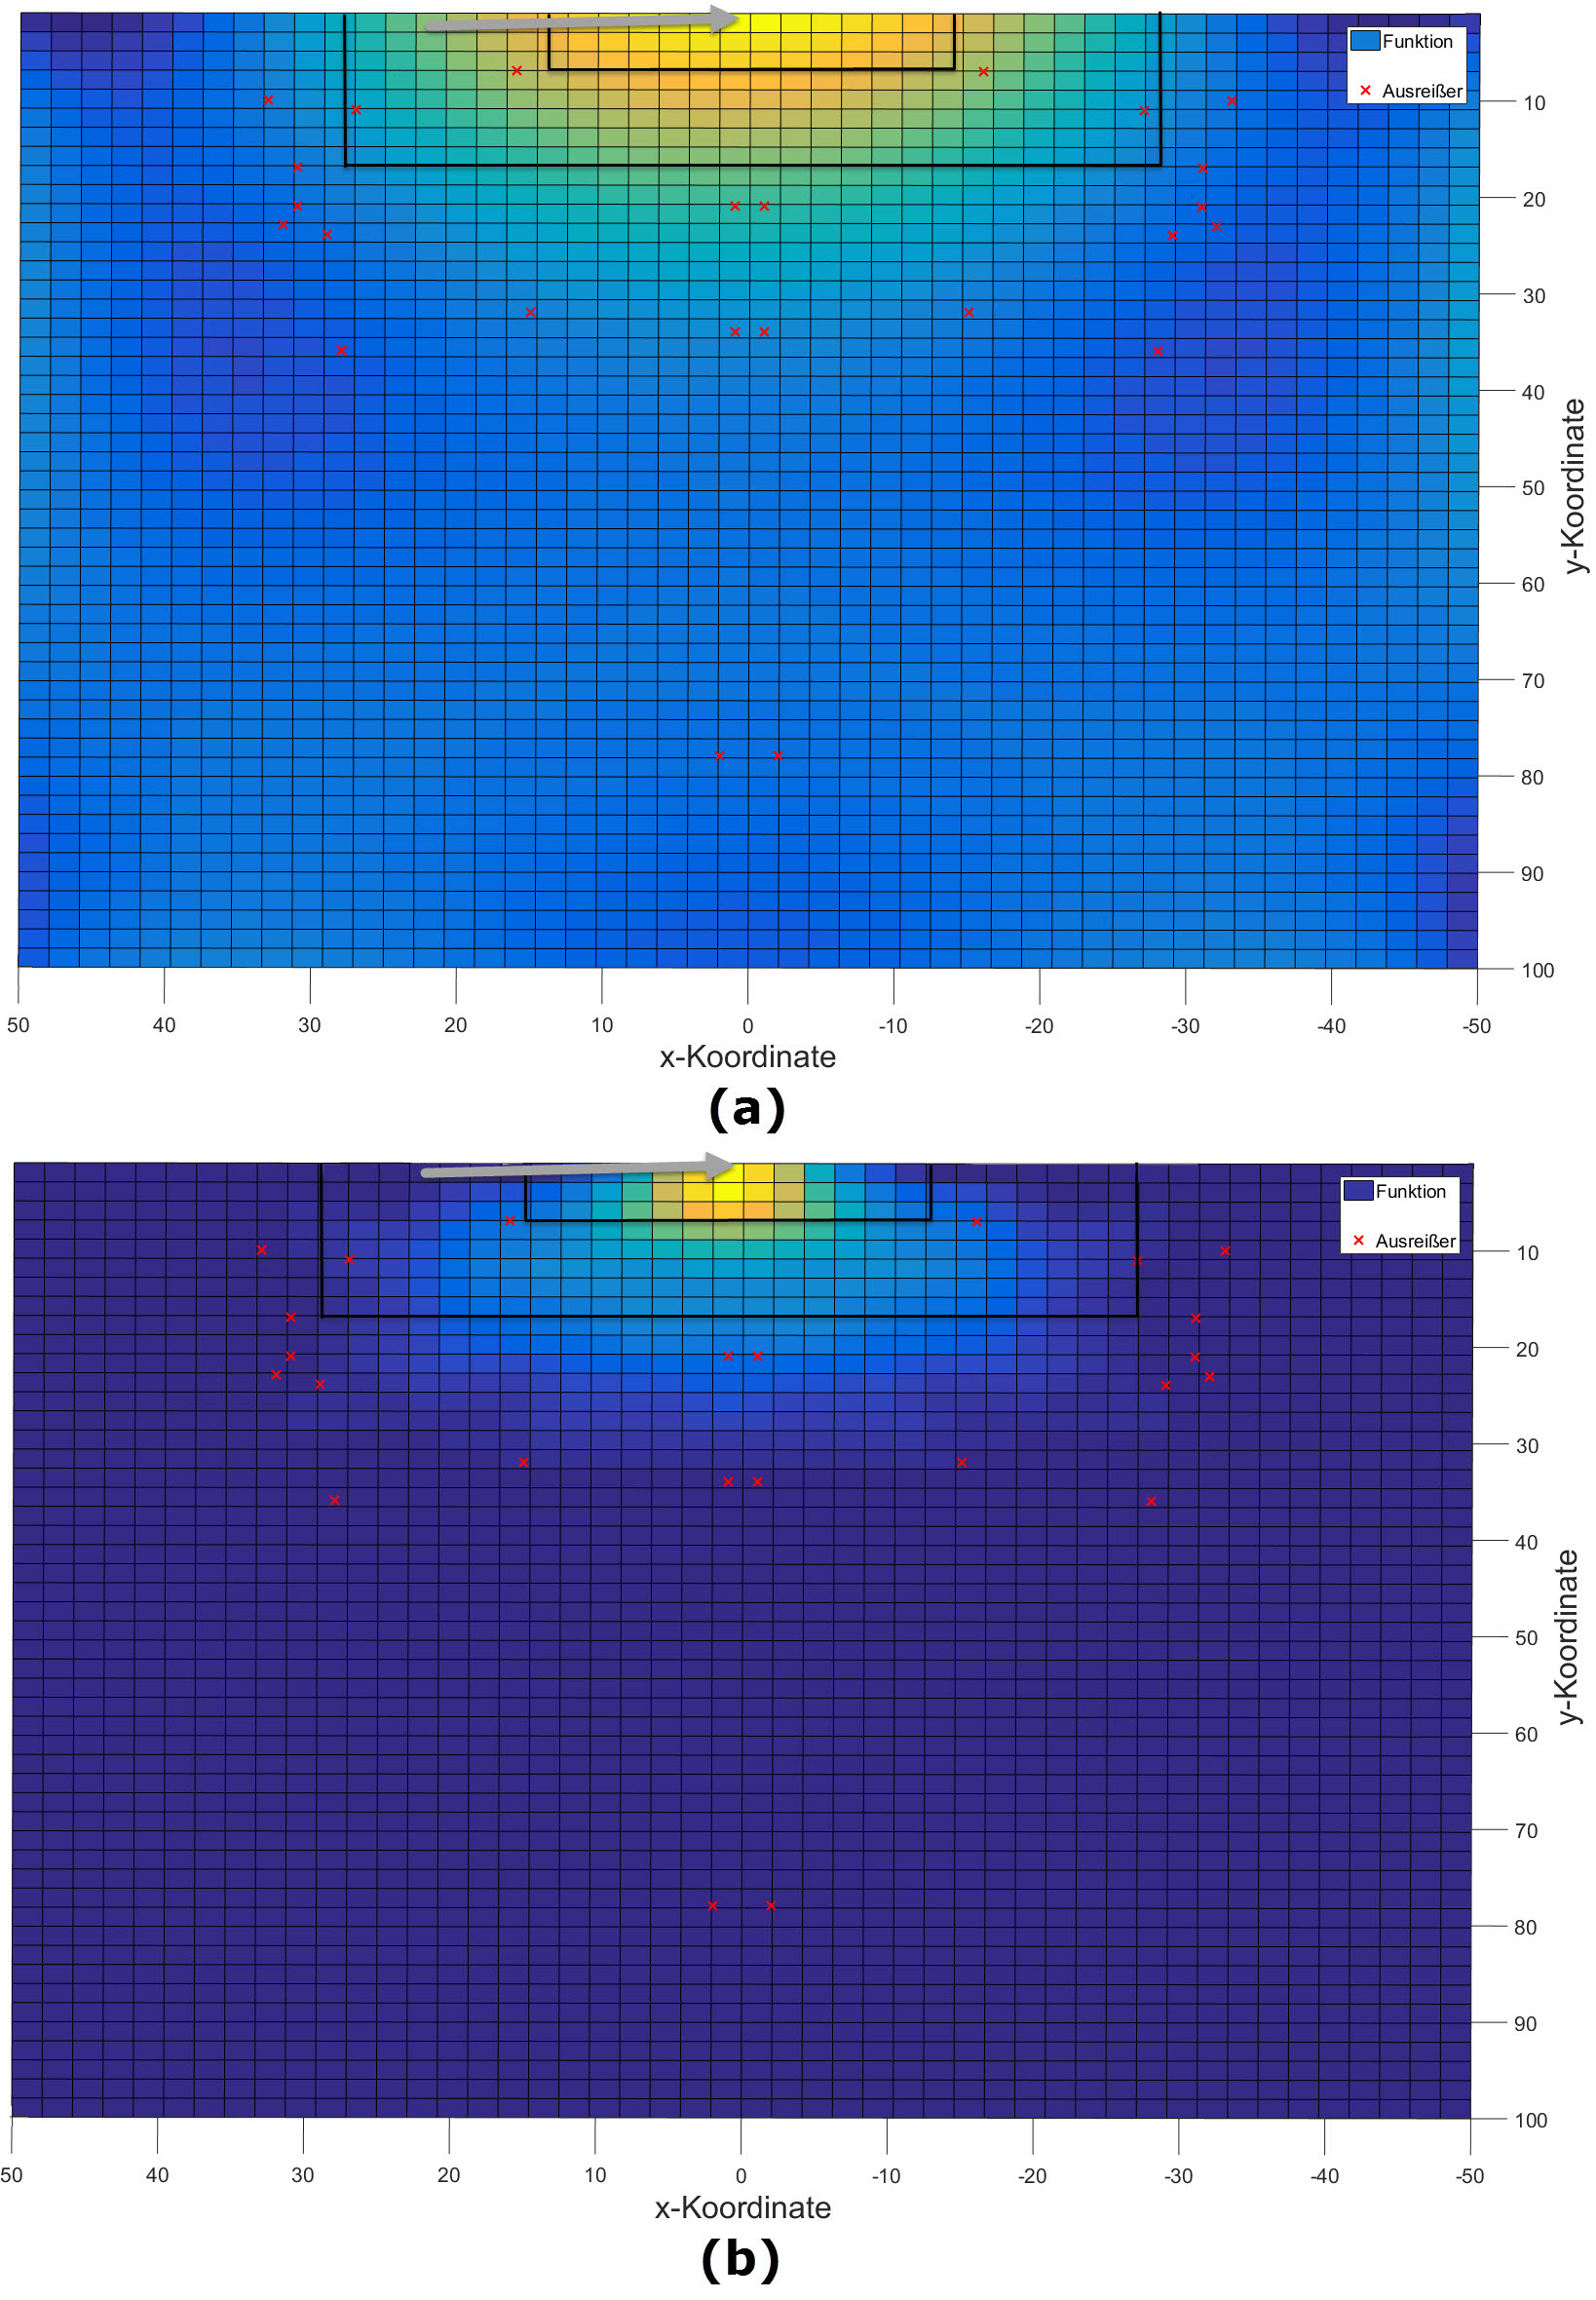
\includegraphics[scale=0.34]{se-wa-jpg/heatmap}
\caption[Vergleich der Regressionsmodelle bei der Koordinatenbetrachtung ]{Vergleich der Regressionsmodelle bei der Koordinatenbetrachtung: (a) Multiple Regression (b) Nichtparametrische Regression}
\label{heatmap}
\end{figure}